\lecture{5}{Feb 5th 10:10}{}
\begin{remark}
    Recall the integration technique for a point \(z\) away from a ring of charge \(q\). 
    \begin{figure}[H]
        \centering
        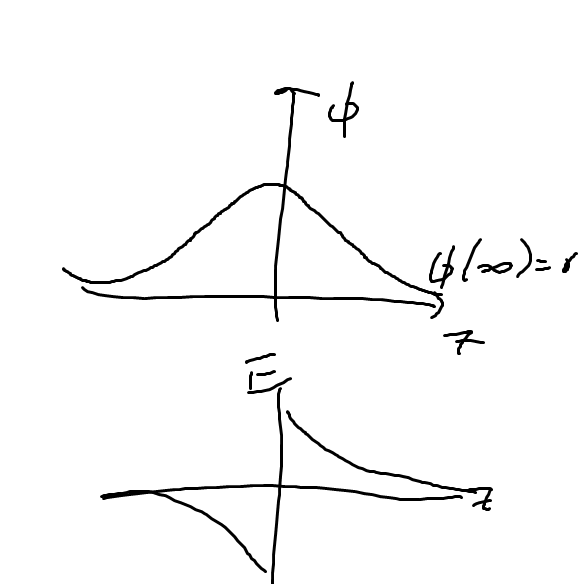
\includegraphics[width=0.8\textwidth]{Figures/01.png}
        \caption{}
        \label{fig:}
    \end{figure}
    This can lead to a generalized conclusion about boundary conditions:
    \begin{eg}
    Condisider a box specifically Gauss's Box:
    \[
        \oint \vec{E} \cdot \hat{n} dS = \sigma \frac{S}{\epsilon }
    \]
    If we look at the coordinates perpendicular to the box which we can denote as 
    \[
        \left( E_{\perp }^{above} - E_{\perp }^{below}     \right) S = \sigma \frac{S}{\epsilon_0}
    \]
    \[
        \left( E_{\perp }^{above} - E_{\perp }^{below} \right) = \frac{\sigma}{\epsilon_0}
    \]
    This is discontinuous and causes the electric field to jump for the perpendicular component. 
    Now we can look at the parellel component with the surface. If we perform the loop integral over the section is that 
    the electric field 
    \[
        \oint \vec{E} \cdot d \vec{l} = 0 
    \]
    which comes from the fact that \(\nabla \times E = 0 \). Thus ew can write that 
    \[
        E_{||}^{above} - E_{||}^{below} = 0   
    \]
    \[
        \vec{E}^{above} - \vec{E}^{below} = \frac{\sigma}{\epsilon _0}  \hat{n} 
    \]
    The potential across the boundary is going to be 
    \[
        \phi^{above} - \phi^{below} = \int_{a}^{b} \vec{E} \cdot d \vec{l} = 0   
    \]
    This tells us that the potential across a charged boundary is still continuous. 
    \end{eg}
    Note that we can convert quantities between \(\phi \) , \(\rho \) , and \(E\) 
    \[
    \phi  = -\int \vec{E} \cdot d \vec{l} 
    \]
    \[
        \nabla ^{2}  \phi  = -\frac{\rho}{\epsilon _0}
    \]
    \[
        \nabla \vec{E}  = \frac{\rho}{\epsilon _0}
    \]
    \[
        \vec{E} = - \nabla \phi 
    \]
    \[
        \vec{E} = \frac{1}{4\pi \epsilon _0} \int \frac{\rho(\vec{r} )}{\vert \vec{r} - \vec{r} ^{\prime}  \vert ^{2}  }dr^{\prime} 
    \]
    \[
        \phi = \frac{1}{4\pi \epsilon _0} \int \frac{\rho(\vec{r} )}{\vec{r} -\vec{r} ^{\prime} } dr^{\prime} 
    \]
\end{remark}

\begin{remark}
    Electrostatic Energy

    The scalar potential is related to the work and energy that we care about. Suppose we wish to move a particle in an electric field 
    from \(p_0 \to  p_1\) where the particle has charge \(q\). What is the work?
    \[
        W = -\int F \cdot d \vec{r} 
    \]
    \[
        W = - \int q \vec{E}  \cdot d \vec{r} 
    \]
    \[
        = q \left[ \phi (p) - \phi (p_0) \right] 
    \]
    Thus we see that the work is independent of the path and that the field \(\vec{E} \) is conservative. 
    If we know the work we can tell the difference to be 
    \[
        \phi (p)-\phi (p_0) = \frac{W}{q}
    \]
    From here we can also know the work needed to assemble a particular charge distribution which is the work needed to assemble a 
    distribution of charges \(q_1, q_2, q_3\). We know that \(\phi (\infty ) = 0\) , so we can move the charges one by one. 
    \(q_1\) has no work done on it to move to the correct place. We then move each aprticle one by one. Thus for \(q_2\) , we have 
    \[
        W_2 = - \int_{\infty }^{r_{12} } q_2 E_1 d \vec{r} = q_2 [\phi (\vec{r}_{12} ) - \phi (\infty )] = q_1 \frac{q_2}{4\pi \epsilon \vert \vec{r_2} - \vec{r_1}  \vert }
    \]
    We can also move the next particle which can be denoted as 
    \[
        W_3 = q_3[\phi (\vec{r}_{13} ) - 0] + q_3[\phi(\vec{r}_{23} )- 0]= (q_1 + q_2 )\frac{q_3}{4\pi \epsilon _0 \vert \vec{r_2} -\vec{r_1}  \vert }
    \]
    \[
        W_{total} = W_3 + W_2 + W_1 
    \]
    we see a structure to calculate the work to be defined to be the work done by 1 to 2, 1 to 3, and 2 to , denoted as 
    \[
        W_{total} = W_{12}+ W_{13} + W_{23}    
    \]
    where 
    \[
        W_{ij} = q_i\frac{q_j}{4\pi  \epsilon_0 \vert \vec{r} _i - \vec{r} _j \vert } 
    \]
    \[
        W_{total} = \sum_{i,j, i \neq j, i < j} W_{ij}   
    \]
    \[
       = \frac{1}{8\pi \epsilon _0} \sum_{i} q_i \sum_{j} \frac{q_i}{\vert \vec{r} _i - \vec{r} _j \vert } 
    \]
    \[
        = \frac{1}{2}\sum_{i} q_i \phi _j (\vec{r} _i) 
    \]
    For a continuous charge distribution we can rewrite this as 
    \[
        W= \frac{1}{8 \pi \epsilon _0} \int _V \int _{V^{\prime}} \frac{\rho (\vec{r} ) \rho ( \vec{r} ^{\prime} )}{\vert \vec{r} -(\vec{r} )^{\prime}  \vert }dV dV^{\prime} 
    \]
    \[
        W= \frac{1}{2} \int _V \rho (\vec{r} )\phi (\vec{r} )dV
    \]
    The energy can then be expressed in terms of work against the Coloumb interaction. Where in another way we can write 
    \[
        W = \frac{1}{2} \int _V \rho (\vec{r} ) \phi (\vec{r} ) dV
    \]
    where the charge density is \(\epsilon _0 (\nabla \cdot\vec{E} )\) 
    \[
        = \frac{1}{2} \int _V e_0 (\nabla \cdot \vec{E} ) \phi dV
    \]
    Notice that 
    \[
    \nabla \cdot (\vec{E}  \phi ) = \nabla \phi  \cdot \vec{E}  + (\nabla  \cdot \vec{E} ) \phi = -\vert E \vert ^{2} + (\nabla  \cdot \vec{E} ) \phi 
    \]
    We can now plug this back and rewrite the work as 
    \[
        W= \frac{1}{2} \int _V \epsilon _0 \left[ \vec{\nabla}  \cdot (\vec{E}  \phi ) + \vert \vec{E}  \vert  ^{2} \right] dV
    \]
    Suppose that the charge is concetrated at a specific point in space. Then we integrate over the entire charge region. We have 
    \[
        \frac{\epsilon_0}{2} \left[  \int _S \phi  \vec{E}  \cdot \hat{n}  dS + \int _V \vert  \vec{E}  \vert  ^{2}  dV\right] 
    \]
    because there are no other charges, we can extend the first term of the surface to be infinitely large. 
    \[
        S \to  r^{2} , \vert  \vec{E}  \vert \to  \frac{1}{r^{2} }, \phi \to \frac{1}{r}
    \]
    Thus the first term is proportional to \(\frac{1}{r^{3} } r^{2}  \to  0\) . Thus we can express the term simply as 
    \[
        W = \frac{\epsilon_0}{2} \int _V \vert \vec{E}  \vert ^{2}  dV
    \]
    We can then denote \(W_e\) as the energy density associated with the electric field. And this is the other form for expressing the potential energy 
    by calculating the electric field squared. Recall the form we had for the first form and there are some inconsisitencies. For the charge density and potential, we can have 
    negative charge density and a positive potential which means the total energy could be negative. On the other term, the term can neber be negative. The 
    way to reconcile this is integrate over a very small space. If we calculate the work to seemble the point charges, the first equation will blow up. 
\end{remark} 